\documentclass{article} % For LaTeX2e
\usepackage{iclr2022_conference,times}
% Optional math commands from https://github.com/goodfeli/dlbook_notation.
%%%%% NEW MATH DEFINITIONS %%%%%

\usepackage{amsmath,amsfonts,bm}

% Mark sections of captions for referring to divisions of figures
\newcommand{\figleft}{{\em (Left)}}
\newcommand{\figcenter}{{\em (Center)}}
\newcommand{\figright}{{\em (Right)}}
\newcommand{\figtop}{{\em (Top)}}
\newcommand{\figbottom}{{\em (Bottom)}}
\newcommand{\captiona}{{\em (a)}}
\newcommand{\captionb}{{\em (b)}}
\newcommand{\captionc}{{\em (c)}}
\newcommand{\captiond}{{\em (d)}}

% Highlight a newly defined term
\newcommand{\newterm}[1]{{\bf #1}}


% Figure reference, lower-case.
\def\figref#1{figure~\ref{#1}}
% Figure reference, capital. For start of sentence
\def\Figref#1{Figure~\ref{#1}}
\def\twofigref#1#2{figures \ref{#1} and \ref{#2}}
\def\quadfigref#1#2#3#4{figures \ref{#1}, \ref{#2}, \ref{#3} and \ref{#4}}
% Section reference, lower-case.
\def\secref#1{section~\ref{#1}}
% Section reference, capital.
\def\Secref#1{Section~\ref{#1}}
% Reference to two sections.
\def\twosecrefs#1#2{sections \ref{#1} and \ref{#2}}
% Reference to three sections.
\def\secrefs#1#2#3{sections \ref{#1}, \ref{#2} and \ref{#3}}
% Reference to an equation, lower-case.
\def\eqref#1{equation~\ref{#1}}
% Reference to an equation, upper case
\def\Eqref#1{Equation~\ref{#1}}
% A raw reference to an equation---avoid using if possible
\def\plaineqref#1{\ref{#1}}
% Reference to a chapter, lower-case.
\def\chapref#1{chapter~\ref{#1}}
% Reference to an equation, upper case.
\def\Chapref#1{Chapter~\ref{#1}}
% Reference to a range of chapters
\def\rangechapref#1#2{chapters\ref{#1}--\ref{#2}}
% Reference to an algorithm, lower-case.
\def\algref#1{algorithm~\ref{#1}}
% Reference to an algorithm, upper case.
\def\Algref#1{Algorithm~\ref{#1}}
\def\twoalgref#1#2{algorithms \ref{#1} and \ref{#2}}
\def\Twoalgref#1#2{Algorithms \ref{#1} and \ref{#2}}
% Reference to a part, lower case
\def\partref#1{part~\ref{#1}}
% Reference to a part, upper case
\def\Partref#1{Part~\ref{#1}}
\def\twopartref#1#2{parts \ref{#1} and \ref{#2}}

\def\ceil#1{\lceil #1 \rceil}
\def\floor#1{\lfloor #1 \rfloor}
\def\1{\bm{1}}
\newcommand{\train}{\mathcal{D}}
\newcommand{\valid}{\mathcal{D_{\mathrm{valid}}}}
\newcommand{\test}{\mathcal{D_{\mathrm{test}}}}

\def\eps{{\epsilon}}


% Random variables
\def\reta{{\textnormal{$\eta$}}}
\def\ra{{\textnormal{a}}}
\def\rb{{\textnormal{b}}}
\def\rc{{\textnormal{c}}}
\def\rd{{\textnormal{d}}}
\def\re{{\textnormal{e}}}
\def\rf{{\textnormal{f}}}
\def\rg{{\textnormal{g}}}
\def\rh{{\textnormal{h}}}
\def\ri{{\textnormal{i}}}
\def\rj{{\textnormal{j}}}
\def\rk{{\textnormal{k}}}
\def\rl{{\textnormal{l}}}
% rm is already a command, just don't name any random variables m
\def\rn{{\textnormal{n}}}
\def\ro{{\textnormal{o}}}
\def\rp{{\textnormal{p}}}
\def\rq{{\textnormal{q}}}
\def\rr{{\textnormal{r}}}
\def\rs{{\textnormal{s}}}
\def\rt{{\textnormal{t}}}
\def\ru{{\textnormal{u}}}
\def\rv{{\textnormal{v}}}
\def\rw{{\textnormal{w}}}
\def\rx{{\textnormal{x}}}
\def\ry{{\textnormal{y}}}
\def\rz{{\textnormal{z}}}

% Random vectors
\def\rvepsilon{{\mathbf{\epsilon}}}
\def\rvtheta{{\mathbf{\theta}}}
\def\rva{{\mathbf{a}}}
\def\rvb{{\mathbf{b}}}
\def\rvc{{\mathbf{c}}}
\def\rvd{{\mathbf{d}}}
\def\rve{{\mathbf{e}}}
\def\rvf{{\mathbf{f}}}
\def\rvg{{\mathbf{g}}}
\def\rvh{{\mathbf{h}}}
\def\rvu{{\mathbf{i}}}
\def\rvj{{\mathbf{j}}}
\def\rvk{{\mathbf{k}}}
\def\rvl{{\mathbf{l}}}
\def\rvm{{\mathbf{m}}}
\def\rvn{{\mathbf{n}}}
\def\rvo{{\mathbf{o}}}
\def\rvp{{\mathbf{p}}}
\def\rvq{{\mathbf{q}}}
\def\rvr{{\mathbf{r}}}
\def\rvs{{\mathbf{s}}}
\def\rvt{{\mathbf{t}}}
\def\rvu{{\mathbf{u}}}
\def\rvv{{\mathbf{v}}}
\def\rvw{{\mathbf{w}}}
\def\rvx{{\mathbf{x}}}
\def\rvy{{\mathbf{y}}}
\def\rvz{{\mathbf{z}}}

% Elements of random vectors
\def\erva{{\textnormal{a}}}
\def\ervb{{\textnormal{b}}}
\def\ervc{{\textnormal{c}}}
\def\ervd{{\textnormal{d}}}
\def\erve{{\textnormal{e}}}
\def\ervf{{\textnormal{f}}}
\def\ervg{{\textnormal{g}}}
\def\ervh{{\textnormal{h}}}
\def\ervi{{\textnormal{i}}}
\def\ervj{{\textnormal{j}}}
\def\ervk{{\textnormal{k}}}
\def\ervl{{\textnormal{l}}}
\def\ervm{{\textnormal{m}}}
\def\ervn{{\textnormal{n}}}
\def\ervo{{\textnormal{o}}}
\def\ervp{{\textnormal{p}}}
\def\ervq{{\textnormal{q}}}
\def\ervr{{\textnormal{r}}}
\def\ervs{{\textnormal{s}}}
\def\ervt{{\textnormal{t}}}
\def\ervu{{\textnormal{u}}}
\def\ervv{{\textnormal{v}}}
\def\ervw{{\textnormal{w}}}
\def\ervx{{\textnormal{x}}}
\def\ervy{{\textnormal{y}}}
\def\ervz{{\textnormal{z}}}

% Random matrices
\def\rmA{{\mathbf{A}}}
\def\rmB{{\mathbf{B}}}
\def\rmC{{\mathbf{C}}}
\def\rmD{{\mathbf{D}}}
\def\rmE{{\mathbf{E}}}
\def\rmF{{\mathbf{F}}}
\def\rmG{{\mathbf{G}}}
\def\rmH{{\mathbf{H}}}
\def\rmI{{\mathbf{I}}}
\def\rmJ{{\mathbf{J}}}
\def\rmK{{\mathbf{K}}}
\def\rmL{{\mathbf{L}}}
\def\rmM{{\mathbf{M}}}
\def\rmN{{\mathbf{N}}}
\def\rmO{{\mathbf{O}}}
\def\rmP{{\mathbf{P}}}
\def\rmQ{{\mathbf{Q}}}
\def\rmR{{\mathbf{R}}}
\def\rmS{{\mathbf{S}}}
\def\rmT{{\mathbf{T}}}
\def\rmU{{\mathbf{U}}}
\def\rmV{{\mathbf{V}}}
\def\rmW{{\mathbf{W}}}
\def\rmX{{\mathbf{X}}}
\def\rmY{{\mathbf{Y}}}
\def\rmZ{{\mathbf{Z}}}

% Elements of random matrices
\def\ermA{{\textnormal{A}}}
\def\ermB{{\textnormal{B}}}
\def\ermC{{\textnormal{C}}}
\def\ermD{{\textnormal{D}}}
\def\ermE{{\textnormal{E}}}
\def\ermF{{\textnormal{F}}}
\def\ermG{{\textnormal{G}}}
\def\ermH{{\textnormal{H}}}
\def\ermI{{\textnormal{I}}}
\def\ermJ{{\textnormal{J}}}
\def\ermK{{\textnormal{K}}}
\def\ermL{{\textnormal{L}}}
\def\ermM{{\textnormal{M}}}
\def\ermN{{\textnormal{N}}}
\def\ermO{{\textnormal{O}}}
\def\ermP{{\textnormal{P}}}
\def\ermQ{{\textnormal{Q}}}
\def\ermR{{\textnormal{R}}}
\def\ermS{{\textnormal{S}}}
\def\ermT{{\textnormal{T}}}
\def\ermU{{\textnormal{U}}}
\def\ermV{{\textnormal{V}}}
\def\ermW{{\textnormal{W}}}
\def\ermX{{\textnormal{X}}}
\def\ermY{{\textnormal{Y}}}
\def\ermZ{{\textnormal{Z}}}

% Vectors
\def\vzero{{\bm{0}}}
\def\vone{{\bm{1}}}
\def\vmu{{\bm{\mu}}}
\def\vtheta{{\bm{\theta}}}
\def\va{{\bm{a}}}
\def\vb{{\bm{b}}}
\def\vc{{\bm{c}}}
\def\vd{{\bm{d}}}
\def\ve{{\bm{e}}}
\def\vf{{\bm{f}}}
\def\vg{{\bm{g}}}
\def\vh{{\bm{h}}}
\def\vi{{\bm{i}}}
\def\vj{{\bm{j}}}
\def\vk{{\bm{k}}}
\def\vl{{\bm{l}}}
\def\vm{{\bm{m}}}
\def\vn{{\bm{n}}}
\def\vo{{\bm{o}}}
\def\vp{{\bm{p}}}
\def\vq{{\bm{q}}}
\def\vr{{\bm{r}}}
\def\vs{{\bm{s}}}
\def\vt{{\bm{t}}}
\def\vu{{\bm{u}}}
\def\vv{{\bm{v}}}
\def\vw{{\bm{w}}}
\def\vx{{\bm{x}}}
\def\vy{{\bm{y}}}
\def\vz{{\bm{z}}}

% Elements of vectors
\def\evalpha{{\alpha}}
\def\evbeta{{\beta}}
\def\evepsilon{{\epsilon}}
\def\evlambda{{\lambda}}
\def\evomega{{\omega}}
\def\evmu{{\mu}}
\def\evpsi{{\psi}}
\def\evsigma{{\sigma}}
\def\evtheta{{\theta}}
\def\eva{{a}}
\def\evb{{b}}
\def\evc{{c}}
\def\evd{{d}}
\def\eve{{e}}
\def\evf{{f}}
\def\evg{{g}}
\def\evh{{h}}
\def\evi{{i}}
\def\evj{{j}}
\def\evk{{k}}
\def\evl{{l}}
\def\evm{{m}}
\def\evn{{n}}
\def\evo{{o}}
\def\evp{{p}}
\def\evq{{q}}
\def\evr{{r}}
\def\evs{{s}}
\def\evt{{t}}
\def\evu{{u}}
\def\evv{{v}}
\def\evw{{w}}
\def\evx{{x}}
\def\evy{{y}}
\def\evz{{z}}

% Matrix
\def\mA{{\bm{A}}}
\def\mB{{\bm{B}}}
\def\mC{{\bm{C}}}
\def\mD{{\bm{D}}}
\def\mE{{\bm{E}}}
\def\mF{{\bm{F}}}
\def\mG{{\bm{G}}}
\def\mH{{\bm{H}}}
\def\mI{{\bm{I}}}
\def\mJ{{\bm{J}}}
\def\mK{{\bm{K}}}
\def\mL{{\bm{L}}}
\def\mM{{\bm{M}}}
\def\mN{{\bm{N}}}
\def\mO{{\bm{O}}}
\def\mP{{\bm{P}}}
\def\mQ{{\bm{Q}}}
\def\mR{{\bm{R}}}
\def\mS{{\bm{S}}}
\def\mT{{\bm{T}}}
\def\mU{{\bm{U}}}
\def\mV{{\bm{V}}}
\def\mW{{\bm{W}}}
\def\mX{{\bm{X}}}
\def\mY{{\bm{Y}}}
\def\mZ{{\bm{Z}}}
\def\mBeta{{\bm{\beta}}}
\def\mPhi{{\bm{\Phi}}}
\def\mLambda{{\bm{\Lambda}}}
\def\mSigma{{\bm{\Sigma}}}

% Tensor
\DeclareMathAlphabet{\mathsfit}{\encodingdefault}{\sfdefault}{m}{sl}
\SetMathAlphabet{\mathsfit}{bold}{\encodingdefault}{\sfdefault}{bx}{n}
\newcommand{\tens}[1]{\bm{\mathsfit{#1}}}
\def\tA{{\tens{A}}}
\def\tB{{\tens{B}}}
\def\tC{{\tens{C}}}
\def\tD{{\tens{D}}}
\def\tE{{\tens{E}}}
\def\tF{{\tens{F}}}
\def\tG{{\tens{G}}}
\def\tH{{\tens{H}}}
\def\tI{{\tens{I}}}
\def\tJ{{\tens{J}}}
\def\tK{{\tens{K}}}
\def\tL{{\tens{L}}}
\def\tM{{\tens{M}}}
\def\tN{{\tens{N}}}
\def\tO{{\tens{O}}}
\def\tP{{\tens{P}}}
\def\tQ{{\tens{Q}}}
\def\tR{{\tens{R}}}
\def\tS{{\tens{S}}}
\def\tT{{\tens{T}}}
\def\tU{{\tens{U}}}
\def\tV{{\tens{V}}}
\def\tW{{\tens{W}}}
\def\tX{{\tens{X}}}
\def\tY{{\tens{Y}}}
\def\tZ{{\tens{Z}}}


% Graph
\def\gA{{\mathcal{A}}}
\def\gB{{\mathcal{B}}}
\def\gC{{\mathcal{C}}}
\def\gD{{\mathcal{D}}}
\def\gE{{\mathcal{E}}}
\def\gF{{\mathcal{F}}}
\def\gG{{\mathcal{G}}}
\def\gH{{\mathcal{H}}}
\def\gI{{\mathcal{I}}}
\def\gJ{{\mathcal{J}}}
\def\gK{{\mathcal{K}}}
\def\gL{{\mathcal{L}}}
\def\gM{{\mathcal{M}}}
\def\gN{{\mathcal{N}}}
\def\gO{{\mathcal{O}}}
\def\gP{{\mathcal{P}}}
\def\gQ{{\mathcal{Q}}}
\def\gR{{\mathcal{R}}}
\def\gS{{\mathcal{S}}}
\def\gT{{\mathcal{T}}}
\def\gU{{\mathcal{U}}}
\def\gV{{\mathcal{V}}}
\def\gW{{\mathcal{W}}}
\def\gX{{\mathcal{X}}}
\def\gY{{\mathcal{Y}}}
\def\gZ{{\mathcal{Z}}}

% Sets
\def\sA{{\mathbb{A}}}
\def\sB{{\mathbb{B}}}
\def\sC{{\mathbb{C}}}
\def\sD{{\mathbb{D}}}
% Don't use a set called E, because this would be the same as our symbol
% for expectation.
\def\sF{{\mathbb{F}}}
\def\sG{{\mathbb{G}}}
\def\sH{{\mathbb{H}}}
\def\sI{{\mathbb{I}}}
\def\sJ{{\mathbb{J}}}
\def\sK{{\mathbb{K}}}
\def\sL{{\mathbb{L}}}
\def\sM{{\mathbb{M}}}
\def\sN{{\mathbb{N}}}
\def\sO{{\mathbb{O}}}
\def\sP{{\mathbb{P}}}
\def\sQ{{\mathbb{Q}}}
\def\sR{{\mathbb{R}}}
\def\sS{{\mathbb{S}}}
\def\sT{{\mathbb{T}}}
\def\sU{{\mathbb{U}}}
\def\sV{{\mathbb{V}}}
\def\sW{{\mathbb{W}}}
\def\sX{{\mathbb{X}}}
\def\sY{{\mathbb{Y}}}
\def\sZ{{\mathbb{Z}}}

% Entries of a matrix
\def\emLambda{{\Lambda}}
\def\emA{{A}}
\def\emB{{B}}
\def\emC{{C}}
\def\emD{{D}}
\def\emE{{E}}
\def\emF{{F}}
\def\emG{{G}}
\def\emH{{H}}
\def\emI{{I}}
\def\emJ{{J}}
\def\emK{{K}}
\def\emL{{L}}
\def\emM{{M}}
\def\emN{{N}}
\def\emO{{O}}
\def\emP{{P}}
\def\emQ{{Q}}
\def\emR{{R}}
\def\emS{{S}}
\def\emT{{T}}
\def\emU{{U}}
\def\emV{{V}}
\def\emW{{W}}
\def\emX{{X}}
\def\emY{{Y}}
\def\emZ{{Z}}
\def\emSigma{{\Sigma}}

% entries of a tensor
% Same font as tensor, without \bm wrapper
\newcommand{\etens}[1]{\mathsfit{#1}}
\def\etLambda{{\etens{\Lambda}}}
\def\etA{{\etens{A}}}
\def\etB{{\etens{B}}}
\def\etC{{\etens{C}}}
\def\etD{{\etens{D}}}
\def\etE{{\etens{E}}}
\def\etF{{\etens{F}}}
\def\etG{{\etens{G}}}
\def\etH{{\etens{H}}}
\def\etI{{\etens{I}}}
\def\etJ{{\etens{J}}}
\def\etK{{\etens{K}}}
\def\etL{{\etens{L}}}
\def\etM{{\etens{M}}}
\def\etN{{\etens{N}}}
\def\etO{{\etens{O}}}
\def\etP{{\etens{P}}}
\def\etQ{{\etens{Q}}}
\def\etR{{\etens{R}}}
\def\etS{{\etens{S}}}
\def\etT{{\etens{T}}}
\def\etU{{\etens{U}}}
\def\etV{{\etens{V}}}
\def\etW{{\etens{W}}}
\def\etX{{\etens{X}}}
\def\etY{{\etens{Y}}}
\def\etZ{{\etens{Z}}}

% The true underlying data generating distribution
\newcommand{\pdata}{p_{\rm{data}}}
% The empirical distribution defined by the training set
\newcommand{\ptrain}{\hat{p}_{\rm{data}}}
\newcommand{\Ptrain}{\hat{P}_{\rm{data}}}
% The model distribution
\newcommand{\pmodel}{p_{\rm{model}}}
\newcommand{\Pmodel}{P_{\rm{model}}}
\newcommand{\ptildemodel}{\tilde{p}_{\rm{model}}}
% Stochastic autoencoder distributions
\newcommand{\pencode}{p_{\rm{encoder}}}
\newcommand{\pdecode}{p_{\rm{decoder}}}
\newcommand{\precons}{p_{\rm{reconstruct}}}

\newcommand{\laplace}{\mathrm{Laplace}} % Laplace distribution

\newcommand{\E}{\mathbb{E}}
\newcommand{\Ls}{\mathcal{L}}
\newcommand{\R}{\mathbb{R}}
\newcommand{\emp}{\tilde{p}}
\newcommand{\lr}{\alpha}
\newcommand{\reg}{\lambda}
\newcommand{\rect}{\mathrm{rectifier}}
\newcommand{\softmax}{\mathrm{softmax}}
\newcommand{\sigmoid}{\sigma}
\newcommand{\softplus}{\zeta}
\newcommand{\KL}{D_{\mathrm{KL}}}
\newcommand{\Var}{\mathrm{Var}}
\newcommand{\standarderror}{\mathrm{SE}}
\newcommand{\Cov}{\mathrm{Cov}}
% Wolfram Mathworld says $L^2$ is for function spaces and $\ell^2$ is for vectors
% But then they seem to use $L^2$ for vectors throughout the site, and so does
% wikipedia.
\newcommand{\normlzero}{L^0}
\newcommand{\normlone}{L^1}
\newcommand{\normltwo}{L^2}
\newcommand{\normlp}{L^p}
\newcommand{\normmax}{L^\infty}

\newcommand{\parents}{Pa} % See usage in notation.tex. Chosen to match Daphne's book.

\DeclareMathOperator*{\argmax}{arg\,max}
\DeclareMathOperator*{\argmin}{arg\,min}

\DeclareMathOperator{\sign}{sign}
\DeclareMathOperator{\Tr}{Tr}
\let\ab\allowbreak


%######## APS360: Uncomment your submission name
\newcommand{\apsname}{Project Proposal}
%\newcommand{\apsname}{Progress Report}
%\newcommand{\apsname}{Final Report}

%######## APS360: Put your Group Number here
\newcommand{\gpnumber}{53}

\usepackage{hyperref}
\usepackage{url}
\usepackage{graphicx}

%######## APS360: Put your project Title here
\title{APS360 Team 53 Project Proposal}


%######## APS360: Put your names, student IDs and Emails here
\author{Shixuan (Shawn) Huang  \\
Student\# 1006964171\\
shixuan.huang@mail.utoronto.ca \\
\And 
Qingran Chen  \\
Student\# 1006724751 \\
qingran.chen@mail.utoronto.ca \\
\AND
Jiahe Lu  \\
Student\# 1007213604 \\
joeyjiahe.lu@mail.utoronto.ca \\
\And
Yunxiang Zhang\\
Student\# 10059850891 \\
vincentyunxiang.zhang@mail.utoronto.ca \\
\AND
}

% The \author macro works with any number of authors. There are two commands
% used to separate the names and addresses of multiple authors: \And and \AND.
%
% Using \And between authors leaves it to \LaTeX{} to determine where to break
% the lines. Using \AND forces a linebreak at that point. So, if \LaTeX{}
% puts 3 of 4 authors names on the first line, and the last on the second
% line, try using \AND instead of \And before the third author name.

\newcommand{\fix}{\marginpar{FIX}}
\newcommand{\new}{\marginpar{NEW}}

\iclrfinalcopy 
%######## APS360: Document starts here
\begin{document}


\maketitle

\begin{abstract}
This project aims to address the pressing issue of deepfake detection within digital media, spotlighting the necessity for advanced verification methods against deceptive content, such as manipulated videos of well-known personalities. Utilizing deep learning techniques, the initiative develops a Convolutional Neural Network (CNN) model to differentiate authentic visuals from fabricated counterparts. The model is honed on a vast and varied image repository provided by Tushar Padhy, aligning with proven detection strategies from significant online challenges and AI security applications. This abstract presents a blueprint for a detection tool that is not only effective in identifying deepfakes but also adheres to ethical data usage and privacy standards.
%######## APS360: Do not change the next line. This shows your Main body page count.
----Total Pages: \pageref{last_page}
\end{abstract}



\section{Introduction}


Deepfake technology, exemplified by unsettling counterfeit videos of celebrities such as Taylor Swift, underscores the necessity of enhancing security measures for online videos and images. This project in focus employs deep learning, an advanced computational approach, to distinguish between realistic and fabricated content. This technical approach is critical due to the potential of deepfakes to deceive individuals and disrupt sectors such as politics and entertainment. The objective of this project is to augment the safety and reliability of online environments, ensuring the integrity of visual content. Through the application of deep learning, the initiative aims to excel in identifying fabricated content, thereby contributing to a more secure internet landscape.


\section{Illustration}
\label{gen_inst}

This project plans to utilize a CNN model to analyze visual imagery. As demonstrated in figure 1, a human face image was first segmented into pixels and used as input for the model. The model then employs a kernel (e.g., a 3×3 matrix) and applies it to the input to extract convolved features. As these features are passed to deeper layers, the model can identify increasingly complex patterns. Ultimately, the features extracted from the CNN and pooling layers are flattened and transformed into learned features. The final output represents the identified features.

\begin{figure}[h]
\begin{center}
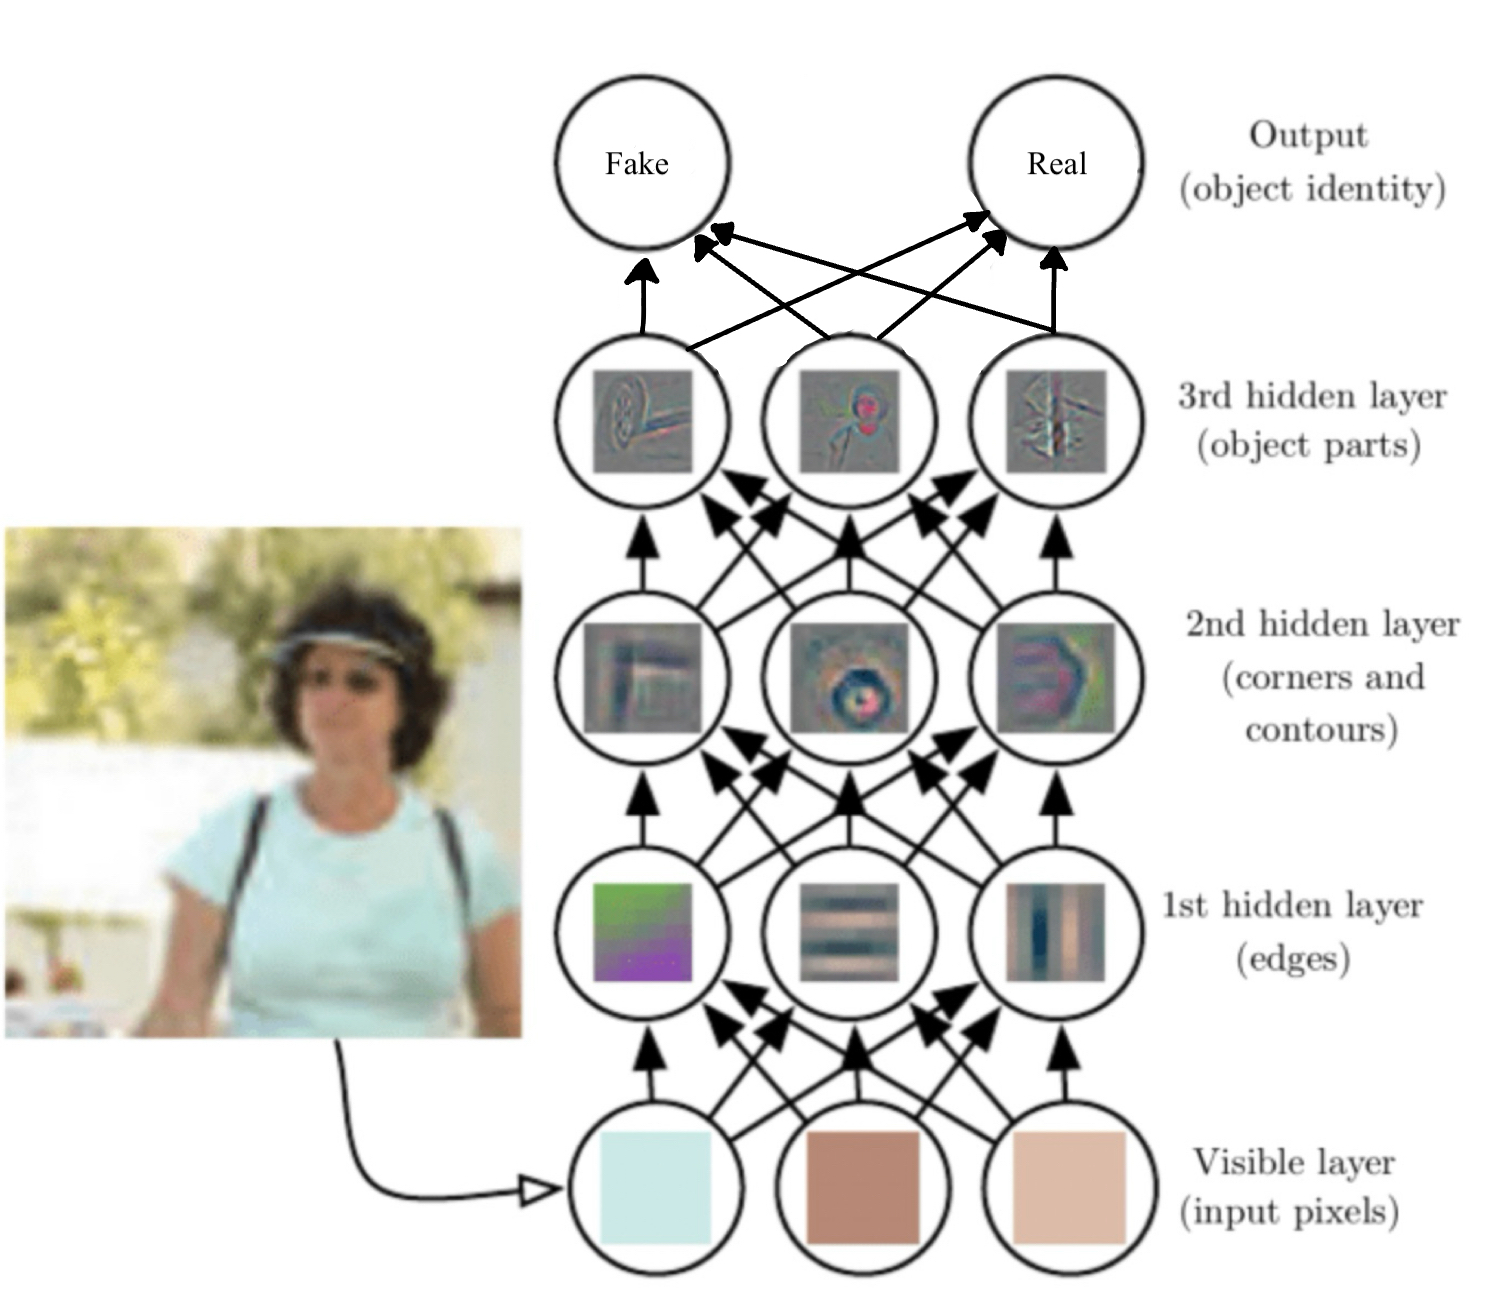
\includegraphics[width=0.6\textwidth]{Figs/cnn.jpg}
\end{center}
\caption{Illustration of CNN model. Image: ~\citep{Mandal_2024}.}
\end{figure}

\section{Background Related Work}
\label{others}

\subsection{Kaggle Deepfake Detection Challenge:}

AWS, Facebook, Microsoft, the Partnership on AI’s Media Integrity Steering Committee, and academics have come together to build the Deepfake Detection Challenge (DFDC) in 2020. ~\citep{Kaggle_DFDC} This competition provides an example of mature criteria for evaluating the model, including the log loss function used for the final model evaluation. The competition also provides a large public database for reference.

\subsection{Sentinel AI:}

Sentinel is a leading AI-based protection platform that helps democratic governments, defence agencies, and enterprises stop the threat of deepfakes. It is used by leading organizations in Europe.  As demonstrated on the website, this large commercial model also uses neural network classifiers, guiding the future development of the model~\citep{Sentinel}.

\subsection{Deepfake detection accuracy by human and machine:}

This paper deeply explores the performance of human, machine, and crowd wisdom when facing DFDC. It collects human decisions through an experimental website, “Detect Fake.” ~\citep{Fake_Deep} The model generally outperforms individual participants, with an accuracy rate of 80 percent compared to participants' rates ranging from 66 to 69 percent. However, when participants accessed the model's predictions, their accuracy increased, indicating potential for human-AI collaboration in enhancing detection capabilities~\citep{Matthew&Zip}.

\subsection{Deepfake Detection Techniques Using Deep Learning: A Survey:}

This paper briefly reviews the deepfake creation and detection technology. It discussed various methods for detection using convolutional neural networks (CNNs), recurrent neural networks (RNNs), and hybrid approaches. The paper also highlights datasets' importance in training, briefly introducing several reliable public datasets~\citep{Almars_2021}.

\subsection{Deepfake Detection with Deep Learning: }

CNN versus Transformers. This paper details the   performance of  eight deep learning architectures (four CNNs and four Transformers) and compares datasets, observing the strengths and uniqueness of the Deeper Forensics, DFDC, and FF++ 2020 datasets. Overall, CNN models did better in the same train-to-test dataset evaluations, and the Transformers models did better in cross-dataset evaluations. Throughout the eight models, the HRNet, XceptionNet, and EfficientNet B7 CNNs models performed very well consistently when trained and tested on the same dataset. In contrast, the XceptionNet, ViT, BeiT, and Swin Transformer performed better in cross-data validation.~\citep{Vrizlynn}

%\subsubsection{}
\section{Data Processing}
\label{others}

In selecting an appropriate dataset for the deep learning model, the collection contributed by Tushar Padhy, comprising over 140,000 portrait images, was selected [7]. This dataset is divided into training, validation, and testing categories, with further segregation into authentic and deepfake images to ensure a balanced representation for in-depth analysis, maintaining a precise 1:1 ratio between the two. Each image is coloured and uniformly set to a resolution of 256x256 pixels, facilitating consistency in the data processing. Importantly, the dataset is characterized by its equitable gender distribution and encompasses a broad spectrum of ages and ethnic backgrounds. It is an exemplary selection for fostering a comprehensive and inclusive model development process. 

The team conducted a visual inspection with random sampling on the dataset across all segments—training, validation, and testing—to identify and remove duplicate images from individuals and across categories, effectively reducing bias and preventing overfitting. The team has emphasized ensuring the authenticity of each image file, eliminating those identified as corrupted. Additionally,  the team has reviewed the dataset to uncover any latent biases towards particular demographic groups. This ensures that the model performs uniformly well across the wide spectrum of ages and ethnic backgrounds represented, maintaining the fairness and dependability of the deepfake detection initiative.

After a comprehensive review of the training, validation, and testing datasets, which revealed no faults or concerns with the images, the team has elected to maintain the original segmentation of these datasets. The team plans to utilize the training set for the development of the model, the validation set for internal testing, and the test set for the ultimate evaluation of the model's performance. The immediate objective is to bolster the model's accuracy in detecting deepfake images by incorporating more training images, subject to the limitations imposed by the project's timeline. It is important to note, however, that the quantity of images integrated into the training process may be revised as the development of the model advances.

\section{Architecture}

This project aims to create a model that detects the deepfake image. In other words, it is an image task classification model. This model consisted of components listed below:

\subsection{Loading the Dataset:}

The model needs to be able to load the cleaned and well-categorized dataset. The model should read these data and be labelled for the output comparison. The team will separate the data into three parts: Training data (used to train the model),  Validation data(to validate the training and discover any overfitting or underfitting and compare with the testing data in the model evaluation), Testing data(to evaluate the model)

\subsection{Training the model and providing results:}

After loading data, the type of neural network needs to be defined. A training function takes in the neural network and trains the model with different hyperparameters. The training should provide two outputs: error(The error rate in training and validating) and loss(Calculating using the choice of loss function to provide how far the prediction is from the expectation). 

\subsection{Plot the training curve:}

Having the training results, the team should plot the training curve and explore whether any overfitting or underfitting exists. To achieve that, the team needs to store the training results in several files on the disk and read from them to plot the training curve.

\subsection{Evaluate the training:}

When the training, analysis, and tuning are complete, the team will evaluate the model using the test data. The evaluation should provide the error rate and loss and be compared with the evaluation of the baseline model.

In this project, the team decided to choose CNN(convolutional neural network) as the neural network:
\begin{description}
  \item[$\bullet$ ] The model is based on image processing and classification. 
  \item[$\bullet$ ] CNN can effectively extract features from images and learn to recognize patterns, making them well-suited for object detection, image segmentation, and classification tasks~\citep{Tripathi_2023}.
  \item[$\bullet$ ] The convolutional layers of CNN can identify the simple features like texture and edges in the lower level and more complex features like objects in the higher level~\citep{Yamashita_2018}. This capability mirrors how humans visualize the picture.
  \item[$\bullet$ ] The same weight(filter) is applied across the whole image, thus allowing the network to search for the same features~\citep{Yamashita_2018}. This parameter sharing significantly reduces the parameters needed to compare with the fully connected networks. It makes CNN more efficient in image processing and less overfitting when processing high-dimensional image data.
  \item[$\bullet$ ] The choice of the loss function will be Binary Cross-Entropy(BCE). The BCE is used for binary classification tasks, where in the model, it will only decide if the image is either deepfaked or not deepfaked (normalized to 0/1). Therefore, BCE is an appropriate choice for the loss function.
\end{description}

\section{Baseline Model}

The initial architecture of the project employs a Convolutional Neural Network (CNN) designed to process and analyze image data efficiently. This baseline model includes several key components, each chosen for its specific contribution to the model's performance:
\begin{description}
  \item[$\bullet$ Convolutional Layer:]  To identify critical features such as textures and edges within the images. The team intends to use 32 filters of size 3x3, a setup that strikes a balance between capturing detailed features and managing computational resources.
  \item[$\bullet$ Activation Function:] The ReLu (Rectified Linear Unit) function is selected due to its effectiveness in adding non-linearity, which is crucial for learning complex patterns. ReLu is favored for its simplicity and ability to mitigate the vanishing gradient problem.
  \item[$\bullet$ Pooling Layer:] A max pooling layer with a 2x2 size follows the convolutional layers to reduce the spatial dimensions of the feature maps. This step is vital for decreasing computational load while retaining the most significant features.
  \item[$\bullet$ Fully Connected Layer: ] This layer integrates the learned features for the final classification. The size of this layer will be adjusted based on the dataset's complexity and the number of output classes to prevent overfitting.
\end{description}

The baseline model is aimed to be simple but eligible as a reference point to compare with the complex model. The developed advanced model is expected to outperform the baseline model (lower error rate and less loss) to justify the model's improvements in performance. This baseline model's architecture is not only geared towards understanding complex visual inputs but also set up to be a comparative standard for evaluating subsequent models. As the model development progresses, alternative models will be compared against this baseline by varying several aspects:
\begin{description}
  \item[$\bullet$ Adjusting Hyperparameters:] The hyperparameters of the baseline model will be set to a default value, where the team will tune the advanced model with different learning rates, batch size, number of layers, the number of filters in convolutional layers, and the size of the fully connected layer. These adjustments can significantly impact the model's learning ability from the dataset. However, both models will be trained with the same number of epochs to be evaluated and visualize how well the advanced model can outperform the baseline model.
  \item[$\bullet$ Changing Functions:] Experiment with different activation functions like Leaky ReLu or sigmoid to assess their impact on model performance.
  \item[$\bullet$ Model Architecture Modifications:] Introducing variations in the architecture, such as adding dropout layers to reduce overfitting or incorporating batch normalization to improve training stability.
\end{description}

The team intends to employ a suite of performance indicators, including accuracy, precision, recall, and the F1 score, for the assessment of these models. Additionally, the computational efficiency and generalization capability of the models will be evaluated by analyzing their performance on a validation set. This strategy aims at enhancing the model's effectiveness and efficiency, ensuring the development of a robust and optimized solution.

\section{Ethical Considerations}

In the pursuit of developing advanced AI models to combat deepfakes, prioritizing the ethical collection and utilization of data, in a manner that honors individual rights, is paramount. The following principles will guide this project:

\subsubsection*{\textbf{Consent Acquisition:}}
 It is essential to obtain explicit consent from individuals before utilizing their images, videos, or audio recordings for AI training purposes. Utilizing personal data without prior authorization is unethical and can lead to dissatisfaction. Commitment to using data exclusively from individuals who have provided explicit consent will be upheld.

\subsubsection*{\textbf{Privacy Protection:}}
Safeguarding the privacy of individuals whose data is utilized is crucial. Efforts will include anonymizing data whenever feasible and ensuring that access is restricted to authorized personnel only. Adherence to privacy regulations such as the GDPR is mandatory, yet the commitment extends beyond legal compliance to a moral obligation to protect personal information.

\subsubsection*{\textbf{Ensuring Equity and Mitigating Bias:}}
 The risk of incorporating biased data, which might not accurately represent diverse populations, thereby introducing unfairness into AI behaviour, is acknowledged. To counteract this, a commitment to utilizing a broad spectrum of data is made, aiming for AI models that are equitable and effective across diverse groups.

\subsubsection*{\textbf{Transparency and Accountability:}}
A commitment to transparency regarding the methods of data collection, utilization, and safeguarding is established. Additionally, there is an acknowledgment of responsibility for the decisions made in the development and application of AI technologies. Openness to acknowledging errors and rectifying them is essential for maintaining public trust.

By adhering to these ethical guidelines, the objective is to not only enhance the AI models' capability in detecting and thwarting deepfakes but also to ensure the approach respects and upholds the dignity and rights of all individuals. The team is dedicated to advancing this project with a commitment to ethical integrity, aiming to contribute positively to the digital environment.

\section{Project Plan}
The internal dealine and milestone for the Project has been settled.See Table~\ref{sample-table}

\begin{table}[t]
\caption{Task Milestone}
\label{sample-table}
\begin{center}
\begin{tabular}{lll}
\multicolumn{1}{c}{\bf Task}  &\multicolumn{1}{c}{\bf People} &\multicolumn{1}{c}{\bf Internal Deadline} 
\\ \hline \\
\textbf{Project Proposal}       \\
\\ \hline \\
Data collection         &Vincent/Isabel  &5/Feb \\
Data cleaning           &Shawn/Joey      &7/Feb \\
Related-Research        &Isabel/Joey     &7/Feb \\
Proposal documentation  &All             &9/Feb \\
\\ \hline \\
\textbf{Progress Report}       \\
\\ \hline \\
CNN model construction         &Vincent/Shawn  &5/Mar \\
Baseline model construction       &Isabel/Joey  &7/Mar \\
Primary Model set up        &Vincent/Shawn  &7/Mar \\
Progress report documentation        &All  &9/Mar \\
\\ \hline \\
\textbf{Project Presentation}       \\
\\ \hline \\
Report Draft         &Shawn/Isabel  &1/Apr \\
PowerPoint Setup        &Vincent/Joey  &3/Apr \\
Recorded Presentation       &All  &3/Apr \\
\\ \hline \\
\textbf{Final Report}       \\
\\ \hline \\
Final Model Testing        &Vincent/Shawn  &5/Apr \\
Data collection         &All  &6/Apr \\
\end{tabular}
\end{center}
\end{table}

\subsection{Way of Working Together}
\begin{description}
  \item[$\bullet$]Team collaboration on coding will be conducted through Google Colab
  \item[$\bullet$]Members must immediately inform the project manager of any issues or delays, along with the work completed so far
  \item[$\bullet$]Weekly meetings will be held for open communication and assignment of coding tasks.
  \item[$\bullet$]To prevent code conflicts, new code blocks should be clearly labeled with their purpose and the author's name.
  \item[$\bullet$]Code should be well-commented for clarity, ensuring easy maintenance and readability.
  \item[$\bullet$]Use Colab's version control to monitor changes; always save a version before significant updates.
  \item[$\bullet$]Team members should proactively share knowledge and provide constructive feedback in the group chat.
  \item[$\bullet$]For conflicts, schedule an urgent meeting for resolution; unresolved issues should be taken to the TA by the project manager or a designated person.
  \item[$\bullet$]Meeting Schedule: Weekly Zoom or Microsoft Teams meetings, with extra meetings arranged as needed.
  \item[$\bullet$]Communication: Team interaction through WeChat, expecting responses within 24 hours for urgent matters.
\end{description}

\section{Risk Register}
Drop-out of member
\begin{description}
  \item[$\bullet$]Task re-assignment: If a member drops out, their workload and responsibilities must be immediately reassessed, and tasks should be reassigned within the team to ensure the smooth progress of the project.
  \item[$\bullet$]Work transfer: Ensure the leaving members have documented and uploaded their work so members can take over their part.
\end{description}
Model-training over time
\begin{description}
  \item[$\bullet$]Change modeling strategy: change current model training strategies like changing the batch size or other hyperparameters
  \item[$\bullet$]Dataset Processing: Check the quality and size of the dataset and try to reduce the dataset's size or optimize the data preprocessing pipeline to speed up training.
  \item[$\bullet$]Internal deadline: set-up internal deadline to prevent emergency issues
\end{description}
Work not finished within the internal deadline
\begin{description}
  \item[$\bullet$]Task reassignment: Evaluate unfinished work and reassign tasks based on priority to ensure that important tasks are completed
  \item[$\bullet$]Priority management: Communicate with relevant team members, reassess project goals and work breakout, negotiate with them to adjust deadlines or reschedule work to ensure the quality and timely completion of work.
\end{description}

\section{Link to GitHub/Colab Notebook}
https://colab.research.google.com/drive/1FIdtQSsjdUm4Gcgm96ySg1RoQFDVHSYs?usp=sharing
Link to Dataset: https://www.kaggle.com/datasets/tusharpadhy/deepfake-dataset 

\label{last_page}

\bibliography{APS360_ref}
\bibliographystyle{iclr2022_conference}

\end{document}
